\begin{figure}
    \centering
    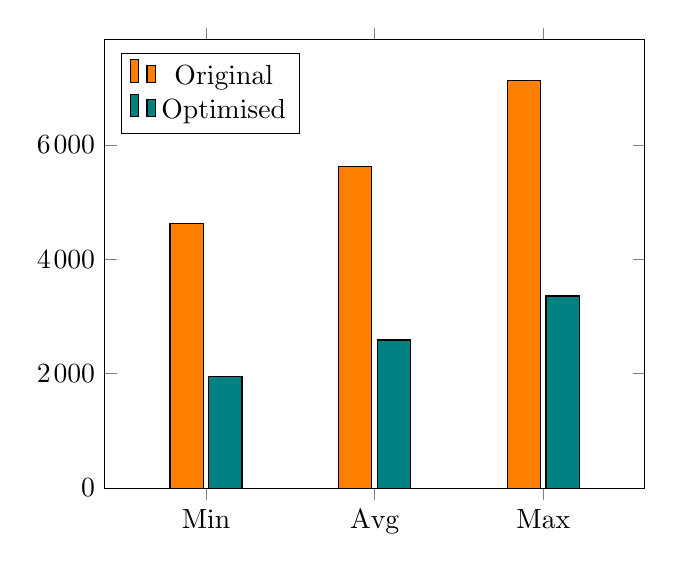
\begin{tikzpicture}
    \begin{axis}[
        ybar,
        bar width=12pt,
        enlarge x limits=0.30,
        /pgf/number format/.cd,
        1000 sep={\hspace{1pt}},
        ymin=0,
        symbolic x coords={Min, Avg, Max},
        xtick=data,
        %nodes near coords,
        legend pos=north west,
    ]
    \addplot[ybar,fill=orange] coordinates {
        (Min,4634)
        (Avg,5628.3)
        (Max,7128)
    };
    \addplot[ybar,fill=teal] coordinates {
        (Min,1955)
        (Avg,2589.5)
        (Max,3359)
        };
    \legend{Original, Optimised}
    \end{axis}
    \end{tikzpicture}
    \caption{\centering{Comparison of number of cycles necessary to deliver 60 packets. The experiment has been done on the basic environment over 10 runs.}}
    \label{fig:meetresultaten}
\end{figure}